%!TEX root = ../my_thesis.tex
\chapter{Results}
\label{chap:results}


\section{Calcite experiment}

In this experiment we will observe the dissolution of calcite ($CaCO_3$) with water. We have decided to choose this reaction because the chemical reaction leading to the dissolution is simple. Moreover, it is an abundant and geologically important material.\cite{hillner1992atomic}\cite{liang1996dissolution} \cite{paquette1995relationship}

The Figure~\ref{fig:calcitegeometry} shows the tilted shape of calcite during dissolution. One part has an angle of 78° and the other 102°\cite{shiraki2000dissolution} \cite{Morse200251}. The shape is tilted because of the different dissolution speed.

\begin{figure}[H]
  \centering
  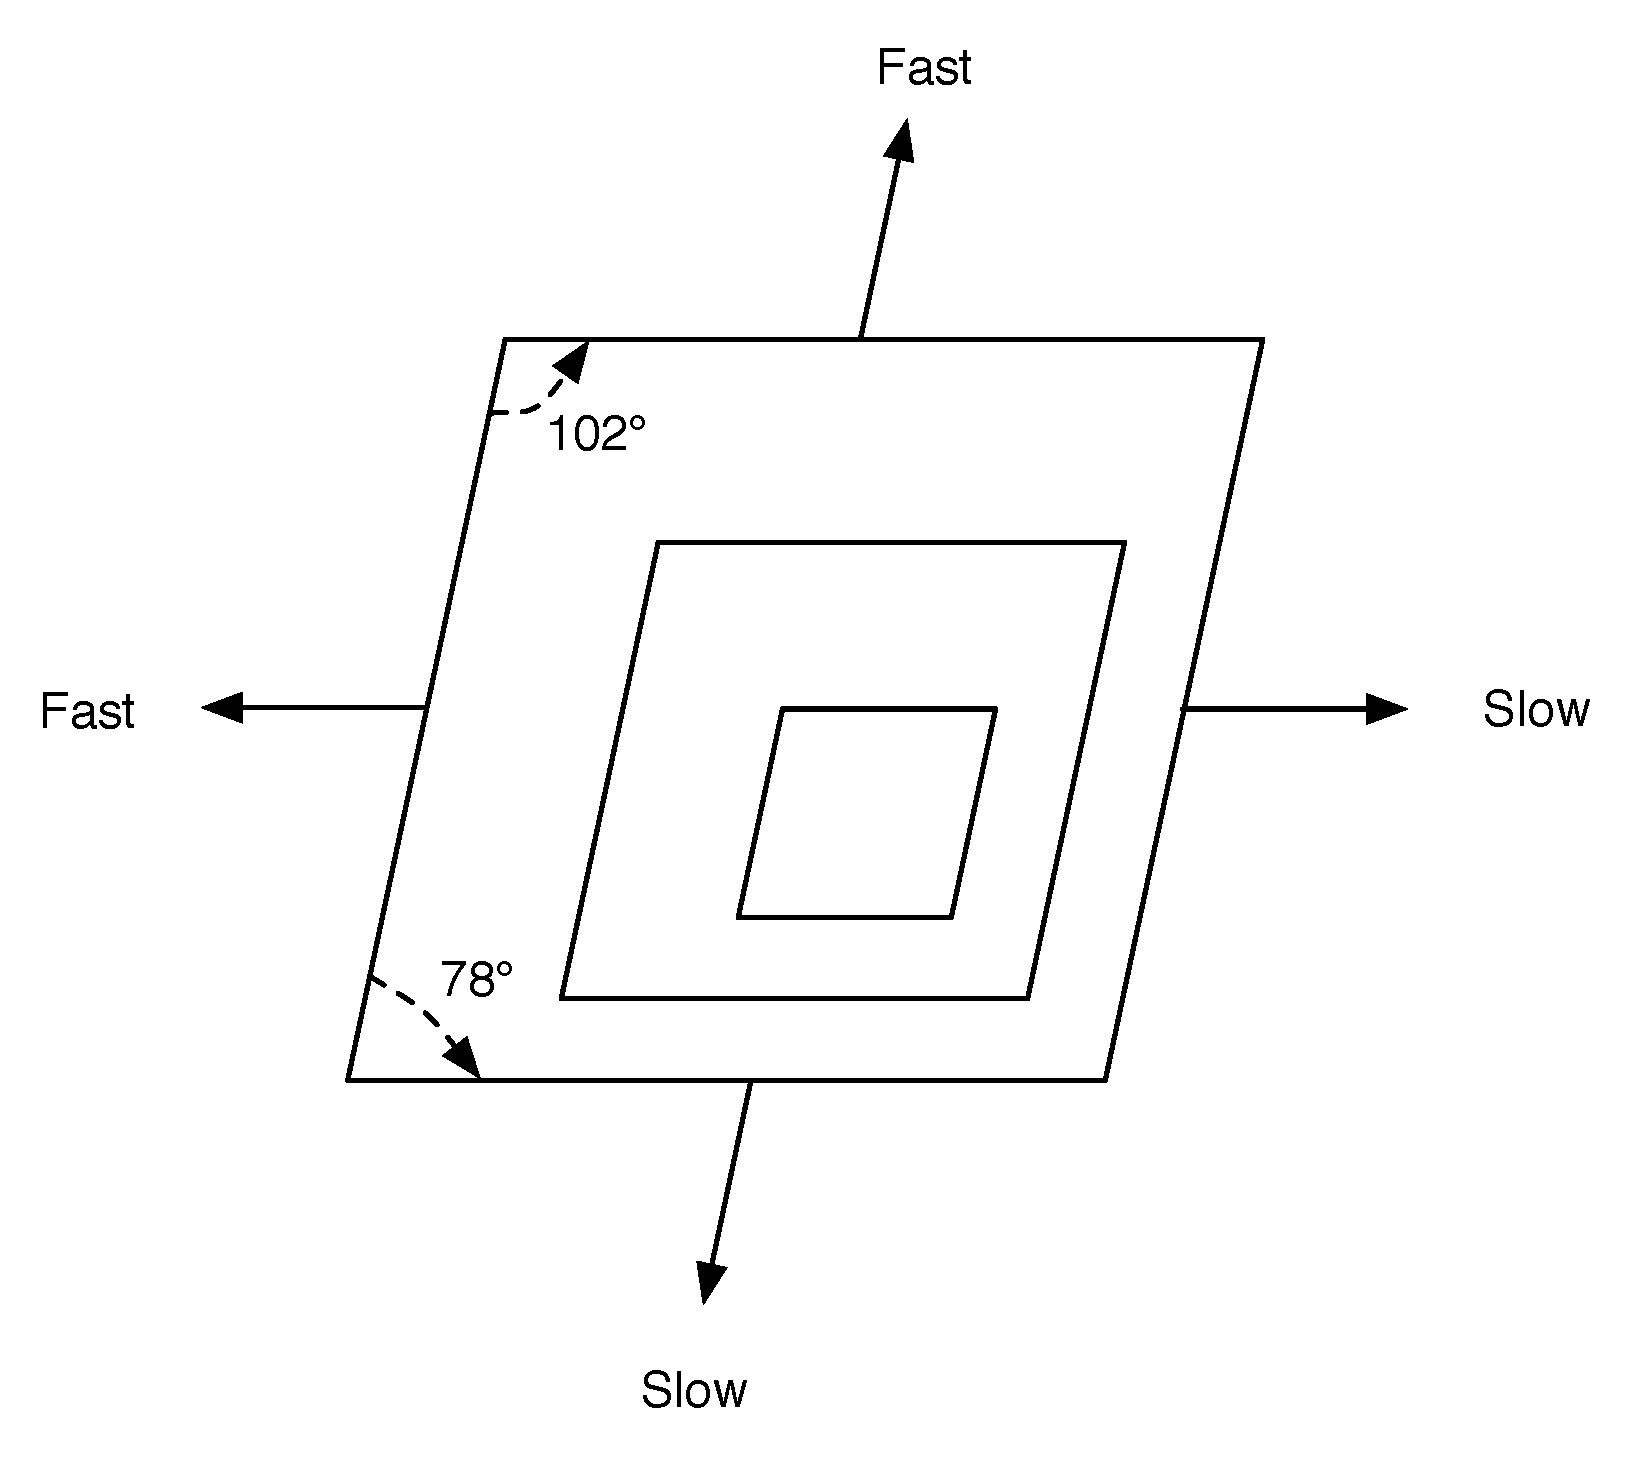
\includegraphics[scale=0.3]{images/calcitegeometry.eps}
    \caption{Calcite geometry}
  \label{fig:calcitegeometry}
\end{figure}
We have used our dual actuators feedback system with a Budget Sensor Tap150-G cantilever. Calcite dissolution is an interesting process to observe with a high speed AFM.
\begin{equation}\label{calcite}
\centering
	CaCO_3(calcite) + H_20 \rightarrow Ca^{2+} + HCO_3^- + OH^- 
\end{equation}
We have mounted our calcite sample on top of the fast piezoelectrical ceramics. Also, we have stuck a plastic cover underneath the piezo for the water. The calcite will dissolve itself with the pattern shown on Figure~\ref{fig:calcitegeometry}. It is linked to its original geometry.
\begin{figure}[H]
  \centering
  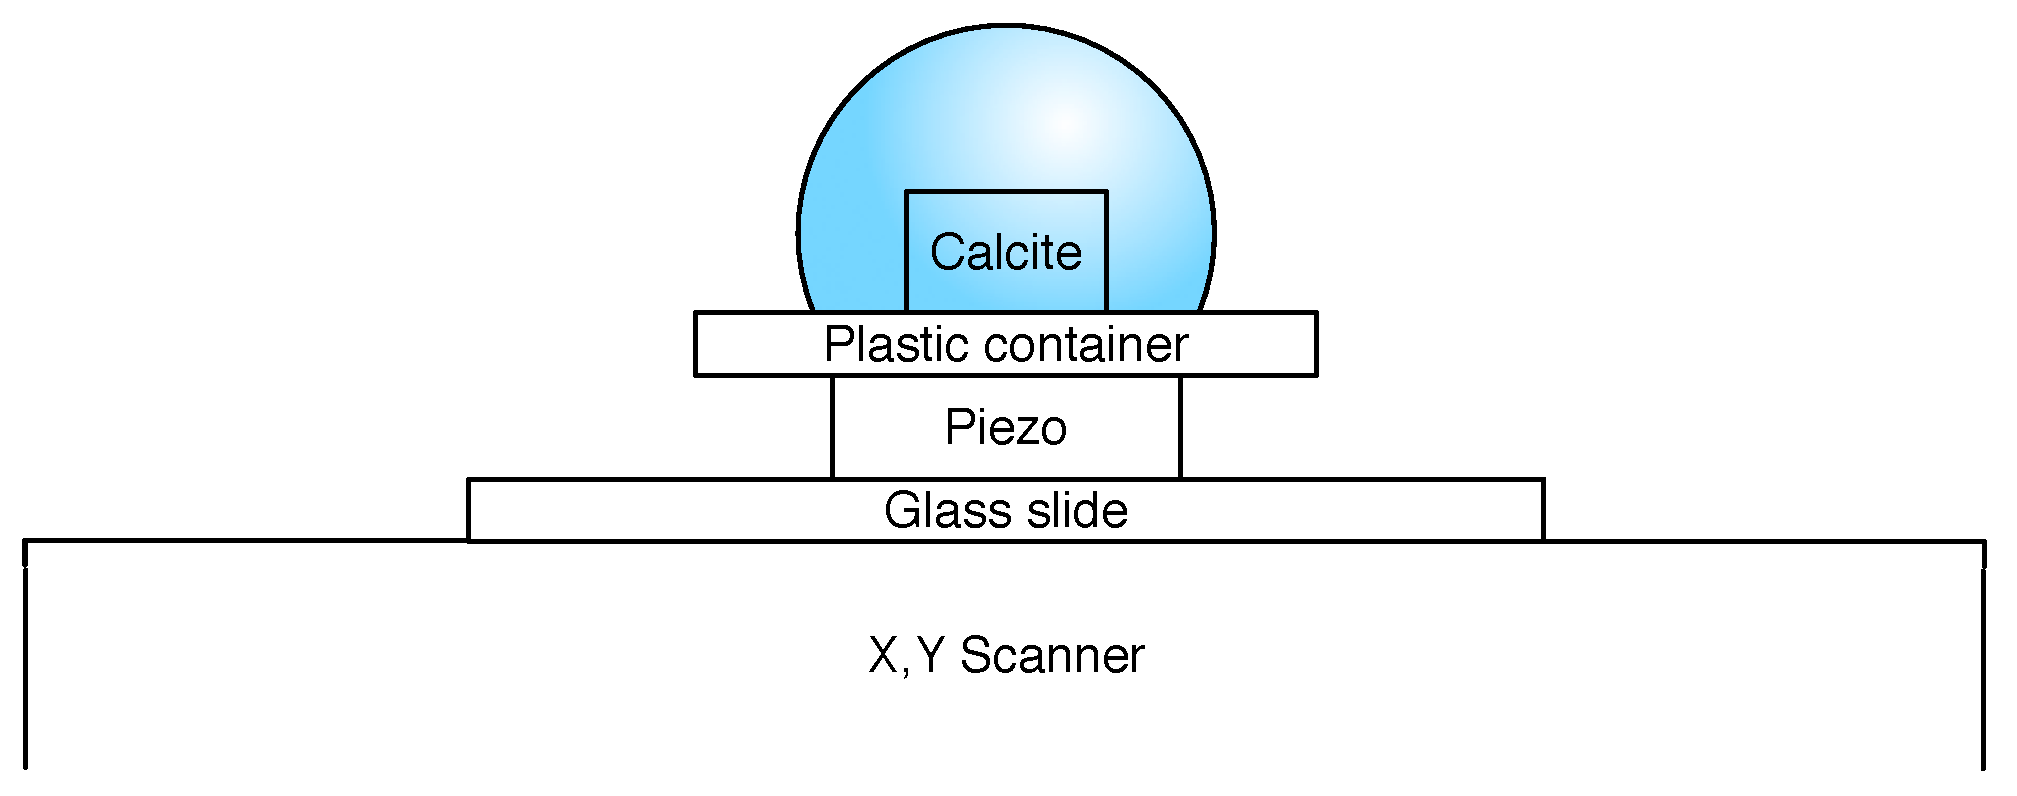
\includegraphics[scale=0.4]{images/calcitesetup.eps}
    \caption{Setup for the calcite experiment}
  \label{fig:calcitesetup}
\end{figure}

We have imaged the same sample with different parameters including scan size, number of spirals and scanning time.


\begin{figure}[!ht]
\centering
\minipage{0.32\textwidth}
    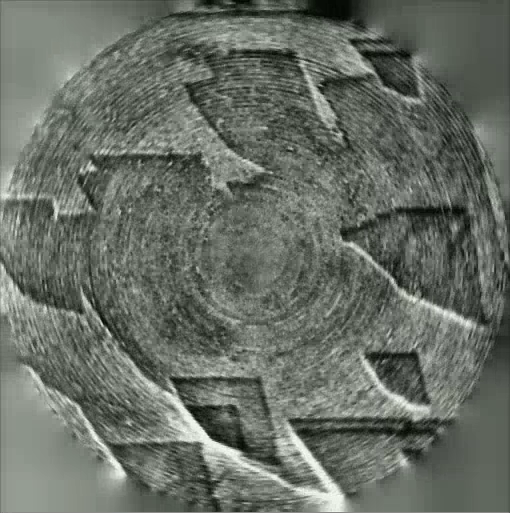
\includegraphics[width=\linewidth]{images/calcite1.png}
    \caption*{t=$t_0$} 
\endminipage\hfill
\minipage{0.32\textwidth}
    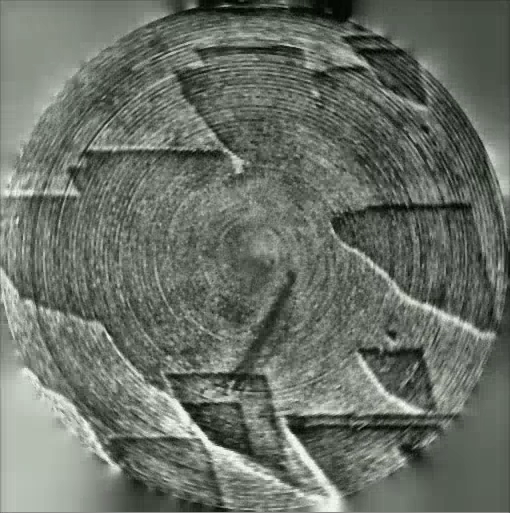
\includegraphics[width=\linewidth]{images/calcite2.png}
    \caption*{t=$t_0$+25s} 
\endminipage\hfill
\minipage{0.32\textwidth}%
    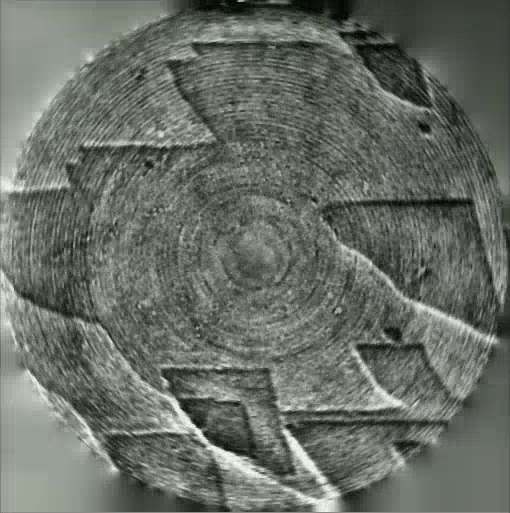
\includegraphics[width=\linewidth]{images/calcite3.png}
    \caption*{t=$t_0$+50s} 
\endminipage
\caption{Evolution of the calcite dissolution over time. 5 $\mu m$ scan size and 100 loops.} \label{fig:cdtotal1}

\end{figure}
The Figure~\ref{fig:cdtotal1} shows the evolution of the calcite. Every scan took 2.5 seconds over a surface of 5 $\mu m$. The scan pattern is an Archimidean spiral with 100 loops and is rendered with heat equation inpainting. We observe the evolution of the front wave over time. After a dozen of minutes, the water will saturate the calcite and the reaction will stop. You can redo the experiment by removing the water and adding fresh water afterwards (Figure~\ref{fig:cdtotal}).


\begin{figure}[!ht]
\centering


\minipage{0.32\textwidth}
    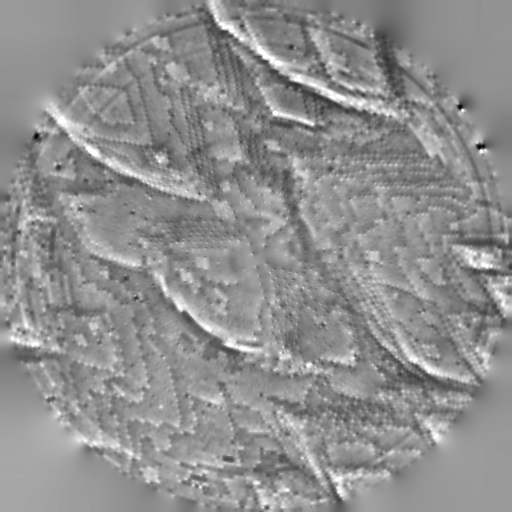
\includegraphics[width=\linewidth]{images/006_X10s50l10m_MOv2_17.png}
    \caption*{t=$t_1$} 
\endminipage\hfill
\minipage{0.32\textwidth}
    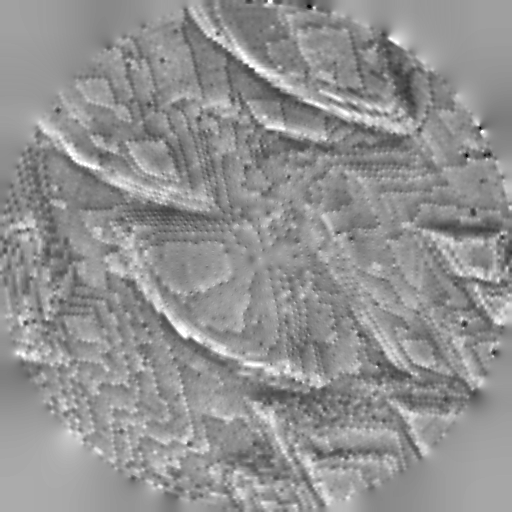
\includegraphics[width=\linewidth]{images/006_X10s50l10m_MOv2_122.png}
    \caption*{t=$t_1$+546s}
\endminipage\hfill
\minipage{0.32\textwidth}%
    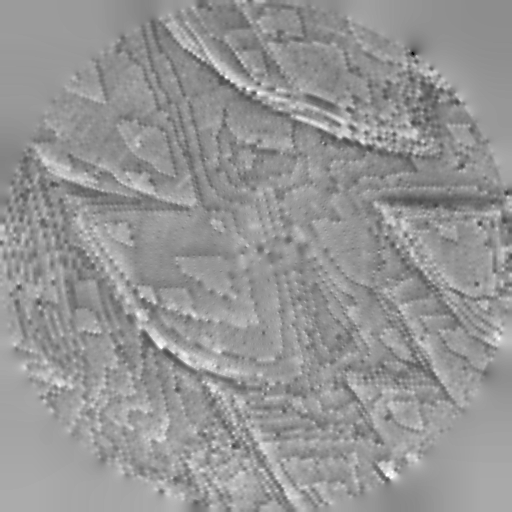
\includegraphics[width=\linewidth]{images/006_X10s50l10m_MOv2_290.png}
    \caption*{t=$t_1$+1,366s} 

\endminipage
\caption{Evolution of the calcite dissolution over time. 10 $\mu m$ scan size and 50 loops.} \label{fig:cdtotal}

\end{figure}


\section{Tilt correction}

In this experiment, we will show the efficiency of the tilt correction. Our sample is a calibration grating with pyramidal features. We use the dual actuators feedback control described in the section~\ref{sec:dualactuator}. Also, the scan pattern is an Archimedean spiral, with a radius of 30 $\mu m$ and 80 loops, described by the equations~\ref{eqarchimedean}.

\begin{equation}\label{eqarchimedean}
x(t)= \alpha \sqrt{t} cos(\beta \sqrt{t})\\
y(t)= \alpha \sqrt{t} sin(\beta \sqrt{t})
\end{equation}

Before applying the tilt correction, we see on the figure~\ref{fig:tiltwaves} a) that our fast piezoelectrical ceramic is saturating. We definitely need to take a load off the actuator.

We have seen in the section~\ref{sec:tiltcompensation} (equation~\ref{eqn:sendwave}) that we need to sample the topography of the surface to compute the plane coefficients. We put a high integral gain for the slow piezo to get the general topography of the sample. The figure~\ref{fig:tiltwaves} b) shows that the surface is not perfectly flat (see z-axis).

Then we compute our fitting algorithm on the x,y and z data of the figure~\ref{fig:tiltwaves} b).


\begin{figure}[!ht]
\centering
\includegraphics[scale=0.2]{images/tiltbigpicture.eps}
\caption{Path on the XY plane}
\label{fig:tiltwaves}
\end{figure}

\begin{table}[H]

\centering % used for centering table
\begin{tabular}{c c c} % centered columns (4 columns)
\hline\hline %inserts double horizontal lines
$a_1$ & $a_2$ & $a_3$ \\ [0.5ex] % inserts table 
%heading
\hline % inserts single horizontal line
-0.14615  & -0.031882 & 29.537 \\[1ex]
\hline %inserts single line
\end{tabular}
\caption{Planefit coefficients} % title of Table
\label{table:planefit} % is used to refer this table in the text
\end{table}

The figure~\ref{fig:spiralztiltout} shows the wave we are going to send to the microscope. The x,y values of the wave's equation (~\ref{eqn:sendwave}) are the output values of the scan pattern.

\begin{figure}[H]
  \centering
  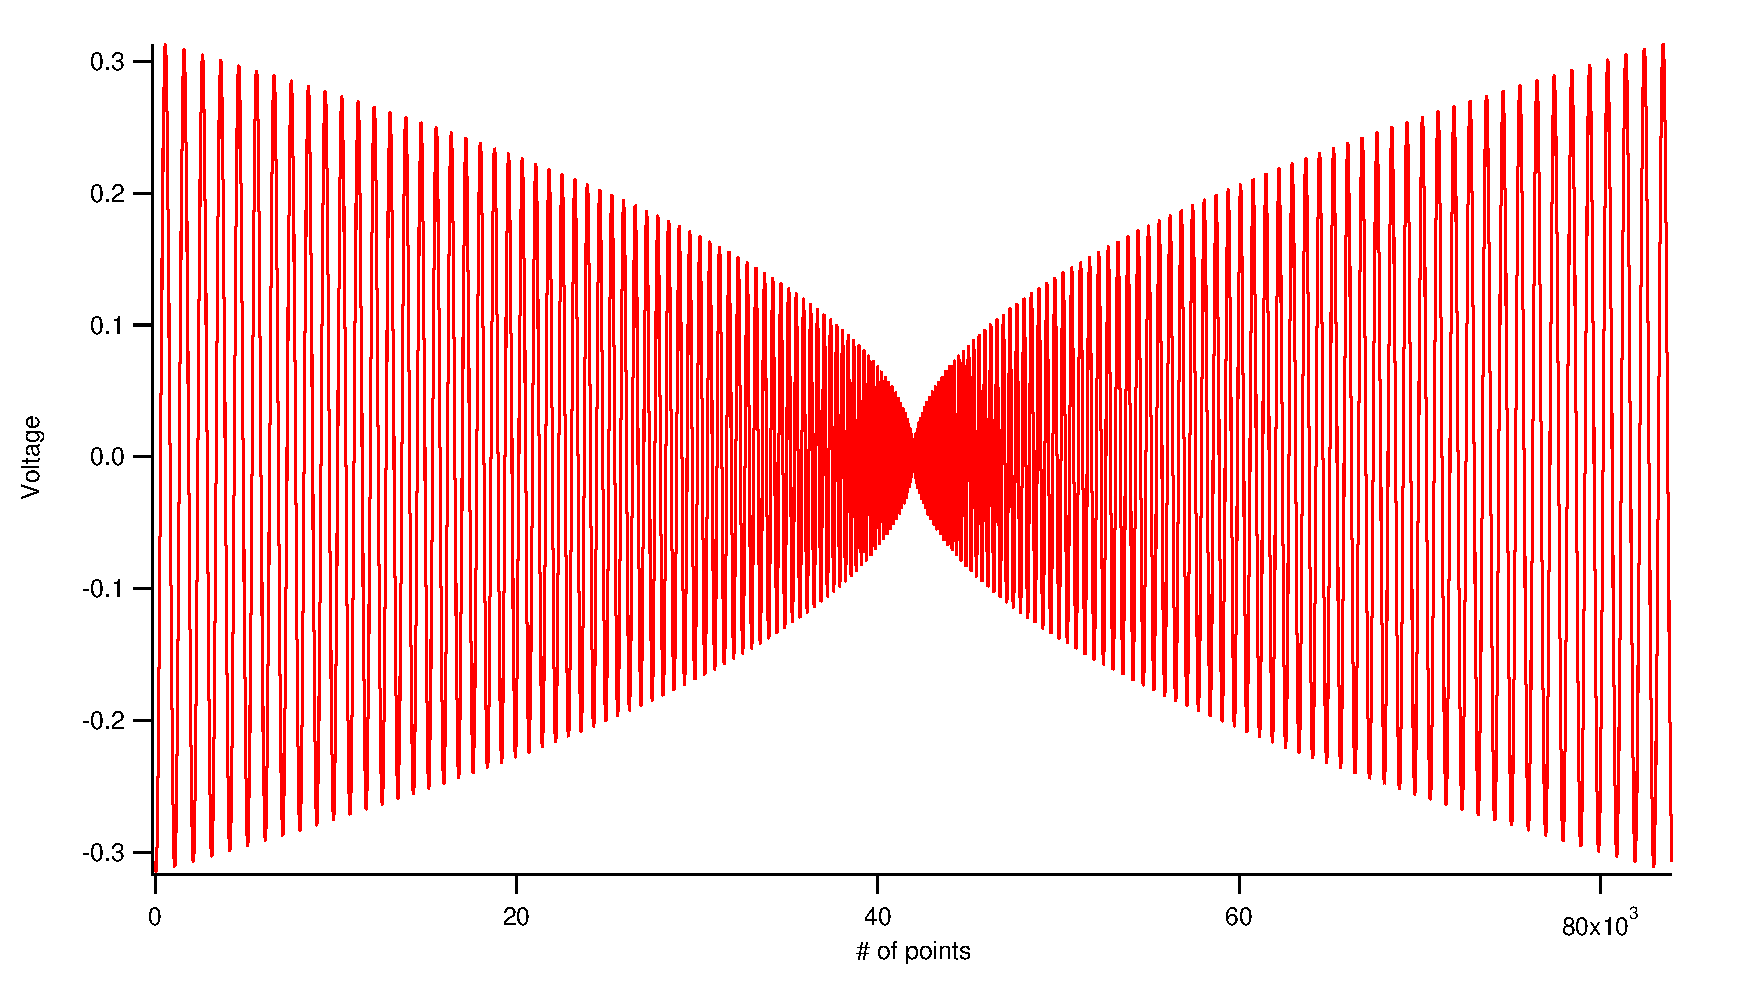
\includegraphics[scale=0.2]{images/spiralztiltout.eps}
    \caption{Input of the tilt compensation}
  \label{fig:spiralztiltout}
\end{figure}

We have calibrated the small piezoelectric ceramic and found that a step of 5V is equal to 180 nm(Input = 2 x calibrationV).

\begin{figure}[!ht]
\begin{minipage}[b]{0.45\linewidth}
\centering
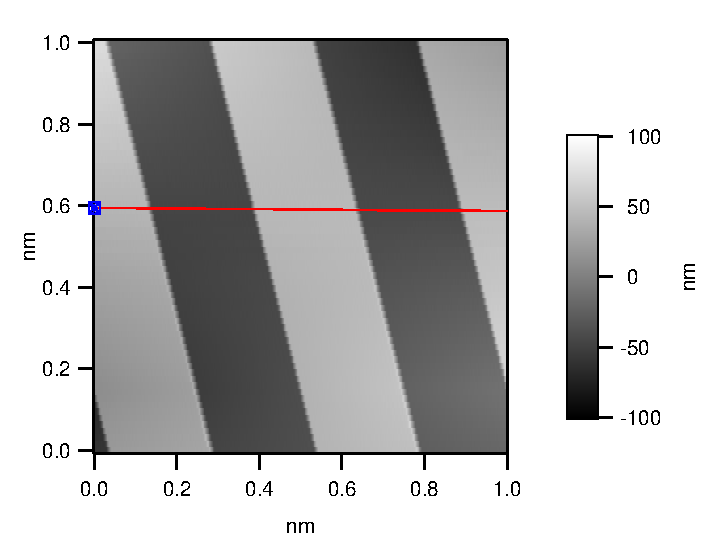
\includegraphics[width=\textwidth]{images/Calib1vPP_HeightMap.eps}
\caption{Height of the calibration}
\label{fig:figure1}
\end{minipage}
\hspace{0.5cm}
\begin{minipage}[b]{0.45\linewidth}
\centering
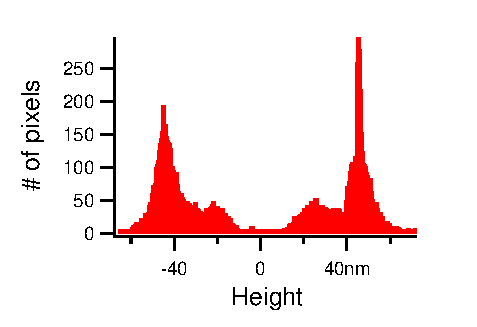
\includegraphics[width=\textwidth]{images/Calib1VppHisto.eps}
\caption{Histogram of the calibration}
\label{fig:figure2}
\end{minipage}
\end{figure}

The tilt compensation takes a load off the small fast piezoelectrical ceramics. The Figure~\ref{fig:tiltimages}  shows the efficiency of our method. Indeed, it was previously saturating. It was trying to reach features that are larger than its range. If we use the tilt correction, we see that it has no problem reaching those features.

\begin{figure}[ht]
\begin{minipage}[b]{0.45\linewidth}
\centering
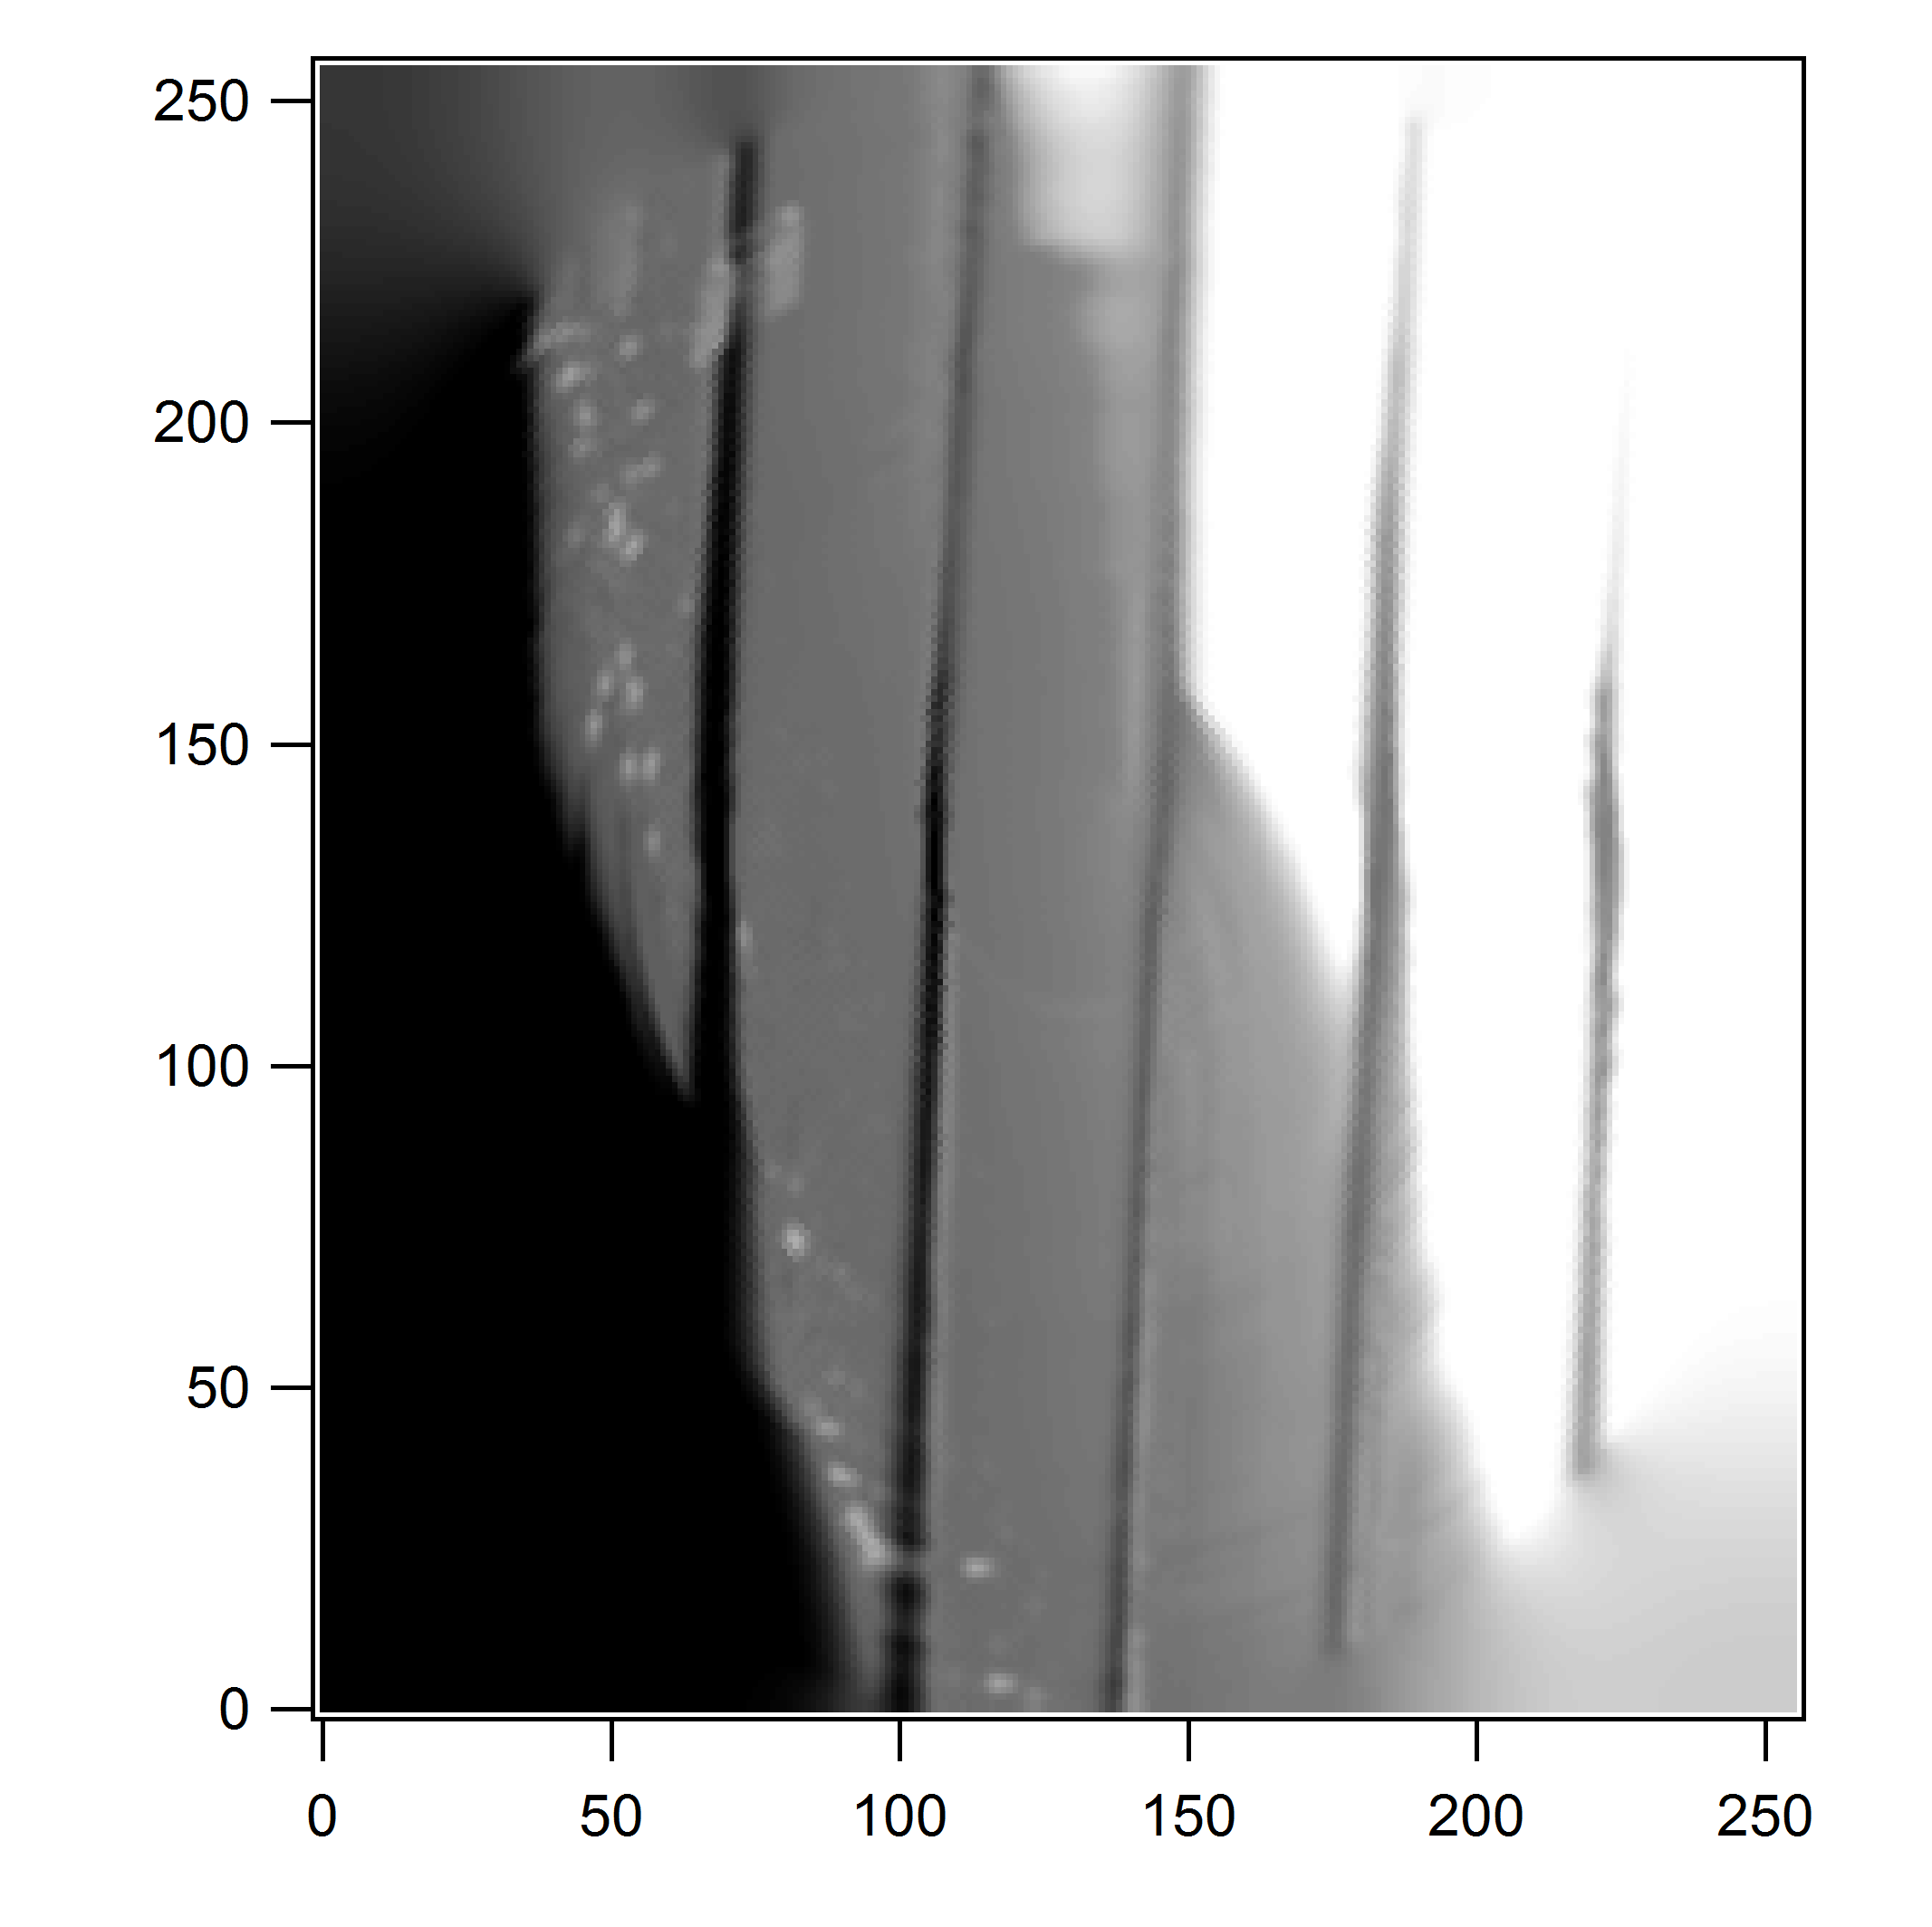
\includegraphics[width=\textwidth]{images/TiltSession0226_27.png}

\end{minipage}
\hspace{0.5cm}
\begin{minipage}[b]{0.45\linewidth}
\centering
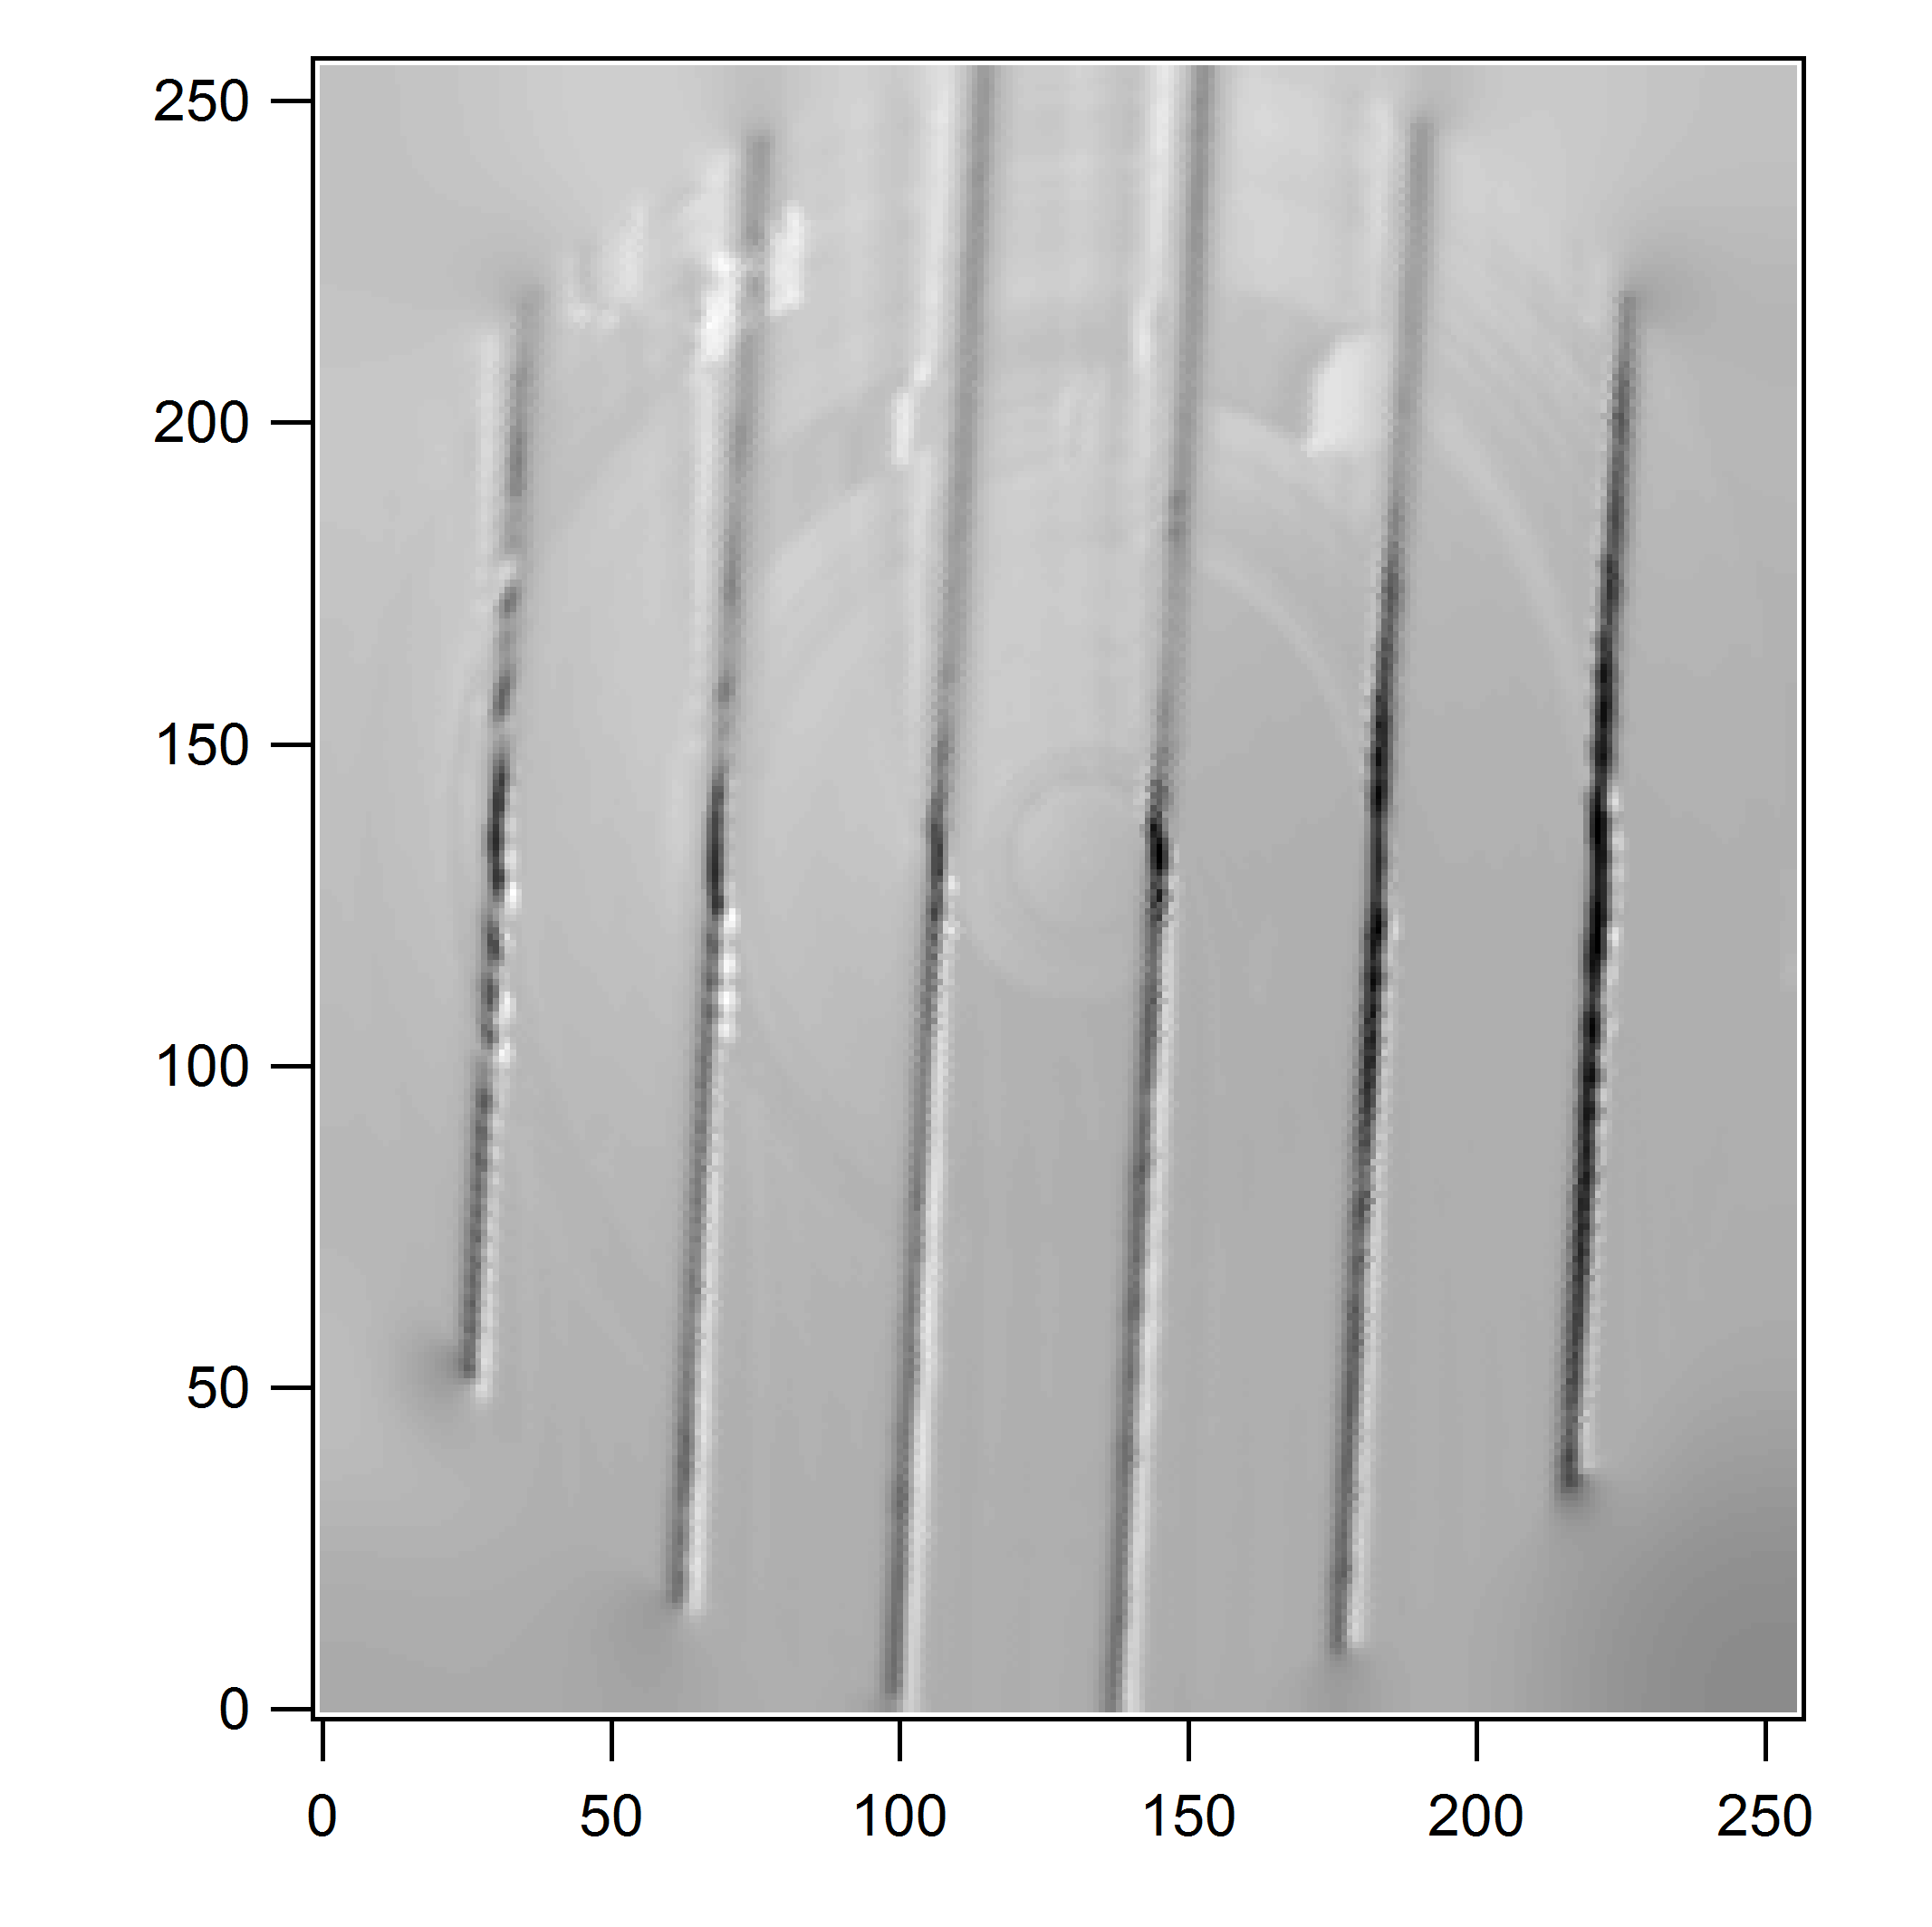
\includegraphics[width=\textwidth]{images/TiltSession0226wc_35.png}
\end{minipage}
\caption{Before and after the tilt correction. The size of the scan is 30 $\mu m$. It has 100 loops and lasted 7.5 seconds}
\label{fig:tiltimages}
\end{figure}



